\section{Background \& Related Work}
\label{sec:RelatedWork}

\subsection{Federated Learning}
\label{subsec:FederatedLearning}

% Intro
In the traditional data-sharing paradigm, multiple institutions collaborate with each other by exchanging or aggregating their data into a central data storage. In contrast, no raw data is exchanged when applying FL. Instead, the data governance stays with each institution, and only models are shared with others.
% Topology, Computing plans
To realize such a collaborative effort, different design choices for FL can be implemented. A distinction can be made on the basis of the topology and the FL compute plan. The topology can be implemented as either centralized or decentralized, meaning the communication is routed via a central server or happens directly between the participants. Popular computing plans are \textit{sequential training}, \textit{peer-to-peer training}, and the usage of an \textit{aggregation server} \citep{Rieke2020TheLearning}.

% Sequential Training
\textit{Sequential training} refers to a training process in which the model is continuously passed on from participant to participant, so each of them waits until the predecessor is finished. The participants can train the model locally for several steps or epochs, depending on the configuration of the training \citep{Chang2018DistributedImaging}. One challenge when applying this computing plan is that it is negatively affected by a phenomenon known as \textit{catastrophic forgetting} \citep{French1999CatastrophicNetworks}, which results in a model highly favoring the data it was trained on most recently.

% Aggregation
The computing plan using an \textit{aggregation server} can be described as follows. At the start of the collaborative training, a machine learning model is sent to all participants. Each replica is individually trained on the locally available data, and then the updated models are sent back to the central server. After receiving the models with their new states, they are aggregated using an aggregation algorithm. The initially proposed is \textit{Federated Averaging} (FedAvg), which is still most widely used today. It computes a weighted average of the received model's parameters, and the resulting consensus model is then again shared with each participant for further training. This process is carried out repeatedly, with each iteration being referred to as a federated round \citep{BrendanMcMahan2017}.

% peer-to-peer
\textit{Peer-to-peer training} can be described as training across multiple nodes without centralization. No central instance exists, and therefore participants communicate directly with each other. This implies that model aggregation itself also takes place on the individual participants.
\textit{Peer-to-peer training} generalizes the approaches of \textit{aggregation server} and \textit{sequential training}. The implementation of such a computing plan can be formed in arbitrary configurations \citep{Chang2018DistributedImaging, Lalitha2019Peer-to-peerGraphs, Roy2019BrainTorrent:Learning}.

% privacy
Although FL provides a basic notion of privacy by keeping the data distributed, additional technical solutions are often required to ensure the privacy and security needed for the clinical application of FL. Kaissis et al. provide an overview of methods for secure and privacy-preserving FL and also possible threats for such learning settings in the field of medical imaging \citep{Kaissis2020SecureImaging}.



\subsection{Federated Learning Solutions}
\label{subsec:SolutionsFL}

% Intro
In order to realize FL, technical solutions are required. One can either use a customized approach for each individual scenario or an existing FL solution. Such FL solutions are presented in the following. %old: It can be a customized approach for each individual scenario or an existing FL solution is used. Such FL solutions are presented in the following.

% NVIDIA Clara Federated
\textbf{NVIDIA Clara Train SDK}
extends the NVIDIA Clara application framework optimized for the healthcare domain. It comes with useful features for medical images and enables developers to train models across institutions. In addition, it has already found some application in academia, as pointed out in the literature review in \Cref{subsec:LitRev} (see page \pageref{subsec:LitRev}). In contrast to other solutions, the source code is not publicly available.

% FATE
\textbf{Federated AI Technology Enabler}\footnote{\url{https://fate.fedai.org/}}
(FATE) is a framework developed as open-source project by FedAI\footnote{\url{https://www.fedai.org/}}, a group of developers of the company WeBank. It provides a secure computing framework to strengthen the federated artificial intelligence ecosystem.
FATE has not yet been applied on medical images in scientific articles.

% FedML
\textbf{FedML}\footnote{\url{https://fedml.ai/}}
is an open research library aiming to facilitate the development of new FL algorithms and fair performance comparison. The solution addresses multiple challenges which occur during scientific research in the field of FL. It is also applicable on edge devices such as smartphones \citep{He2020FedML:Learning}.
So far, FedML has not been used in academic articles on FL using medical images.

% Openmined / PySyft
\textbf{PySyft}\footnote{\url{https://github.com/OpenMined/PySyft}}
is a privacy-preserving FL solution which is originally built over PyTorch but also supports implementations in TensorFlow. It aims to enable developers to write software which can compute over data which is not locally available but on remote machines they do not control. It comes with a large and active open-source community named Openmined\footnote{\url{https://www.openmined.org/}} which is continuously enhancing the solution \citep{Ryffel2018ALearning}. As shown in \Cref{subsec:LitRev} (see page \pageref{subsec:LitRev}), PySyft has already been used in relevant research articles.

% PaddleFL
\textbf{PaddleFL}\footnote{\url{https://github.com/PaddlePaddle/PaddleFL}}
(PFL) is a solution based on PaddlePaddle (PP), a DL framework developed by the company Baidu. PFL benefits from the underlying PP being a distributed and scalable platform with advanced functionalities.
%One must note that only a small amount of resources is available in English, which makes it difficult to use, to fully understand, and to evaluate the solution.
PFL has not yet been used in published research on FL with medical images.

% TensorFlow Federated
\textbf{TensorFlow Federated}\footnote{\url{https://www.tensorflow.org/federated}}
(TFF) extends TensorFlow to facilitate open research and experimentation with FL in a simulated environment. It comes with two application programming interfaces (APIs): FL API and Federated Core API. Both represent different layers that can be adapted and extended by developers. By providing a multi-machine simulation runtime, TFF can be used for FL experiments applying different algorithms. As TensorFlow itself, TFF is an open-source project. So far, TFF has not been used in academic articles on FL using medical images.

% Disclaimer
Please note that further solutions may exist. In our understanding, the above-mentioned are the most promising and well-known solutions and have already been examined in other publications \citep{Li2019AProtection, He2020FedML:Learning}.



\subsection{Federated Learning with Medical Image Data}
\label{subsec:LitRev}

% Literature Search, search query etc.
We systematically performed a literature search to identify publications applying FL on medical images. The basis for our search is the work of \cite{Kirienko2021DistributedAI}. The authors applied the search term \textit{``distributed learning'' or ``federated learning''} on the EMBASE and PubMed/MEDLINE databases. Out of the 26 articles identified, six applied FL using medical image data and are therefore relevant for our research context. Contributions up to July 21, 2020 were taken into consideration. We adopted the applied search procedure and extended the time period until May 31, 2021, resulting in 146 initial hits. After removing duplicates and initial screening of titles and abstracts, eight articles remained. Through forward and backward search, four additional articles were identified. Together with two previously known articles of \cite{Wang2020AutomatedLearning} and \cite{Roth2020FederatedImplementation} and the results selected from \cite{Kirienko2021DistributedAI}, this adds up to 20 articles applying FL on medical images.

% Literature Review: analysis
The articles were analyzed regarding the following characteristics: used FL setting, FL solution, number of participants, computing plan, used algorithm, and given task. We differentiate between three types of FL environments: \textit{real-world}, \textit{synthetic}, and \textit{simulated}.  We differentiate between three types of FL setting: \textit{real-world}, \textit{synthetic}, and \textit{simulated}.
% real-world
A setting that trains a model across geographically distributed institutions is referred to as \textit{real-world}.
% synthetic
Articles were classified as \textit{synthetic} if a FL solution imitates a distributed system technically, by using multiple workers or computation units, such as individual servers, without having an actual

\begin{sidewaystable}[htbp]
%\begin{adjustbox}{width=1.0\textwidth}
\begin{adjustbox}{width=1.0\textheight}
  \centering
  \begin{tabular}{cccccccc}
    Reference & FL Setting & FL Solution & Participants & Computing Plan & Algorithm & Task \\
    \hline \\[-2.5ex] %[-1.5ex]
    \cite{Xu2020ADiagnosis}                             & real-world & custom solution          & 4             & FedAvg                    & 3D-Densenet       & Classification \\
    \cite{Balachandar2020AccountingImaging}             & simulated  & -                        & 4             & Sequential                & GoogleLeNet       & Classification \\
    \cite{Wang2020AutomatedLearning}                    & real-world & NVIDIA Clara Federated   & 2             & FedAvg                    & C2FNAS            & Segmentation \\
    \cite{Remedios2020DistributedSegmentation}          & real-world & custom solution          & 2             & Sequential                & U-Net             & Segmentation  \\
    \cite{Remedios2019DistributedInjury}                & real-world & custom solution          & 2             & Sequential                & CNN (Incept.)     & Segmentation  \\
    \cite{Chang2018DistributedImaging}                  & simulated  & -                        & 4             & Sequential \& Ensembling  & ResNet34          & Classification \\
    \cite{Kaissis2021End-to-endImaging}                 & synthetic  & PriMIA (based on PySyft) & 3             & FedAvg                    & ResNet18          & Classification  \\
    \cite{Dou2021FederatedStudy}                        & synthetic  & custom solution          & 3             & FedAvg                    & CNN               & Segmentation \\
    \cite{Roth2020FederatedImplementation}              & real-world & NVIDIA Clara Federated   & 7             & FedAvg                    & DenseNet-121      & Classification \\
    \cite{Feki2021FederatedImages}                      & simulated  & -                        & 4             & FedAvg                    & VGG16 \& ResNet50 & Classification \\    
    \cite{Sarma2021FederatedSharing}                    & real-world & NVIDIA Clara Federated   & 3             & FedAvg                    & 3D AH Net         & Segmentation \\
    \cite{Sheller2020FederatedData}                     & simulated  & -                        & 10            & FedAvg \& Sequential      & U-Net             & Segmentation \\
    \cite{Baheti2020FederatedNodules}                   & simulated  & -                        & 3             & FedAvg                    & V-Net             & Classification \\    
    \cite{Yang2021FederatedJapan}                       & synthetic  & NVIDIA Clara Federated   & 3             & FedAvg                    & 3D U-Net          & Segmentation \\  
    \cite{Sheller2019Multi-institutionalSegmentation}   & simulated  & -                        & 4, 6, 8, 32   & FedAvg                    & U-Net             & Segmentation \\
    \cite{Li2019Privacy-preservingSegmentation}         & synthetic  & NVIDIA Clara Federated   & 13            & FedAvg                    & CNN               & Segmentation \\
    \cite{Andreux2020SiloedDatasets}                    & simulated  & -                        & 2, 5          & FedAvg                    & CNN               & Segmentation \\
    \cite{Yan2020Variation-AwareData}                   & simulated  & -                        & 2, 4, 8       & FedAvg                    & CNN               & Classification \\
    \cite{Lee2021FederatedEnvironment}                  & real-world & PySyft                   & 6             & FedAvg                    & multiple          & Classification \\
    \cite{Flores2021FederatedPatients}\rlap{*}          & real-world & NVIDIA Clara Federated   & 20            & FedAvg                    & ResNet34          & Classification \\
  \end{tabular}
  \end{adjustbox}
  \caption[Identified articles applying FL using medical image data]{List of identified articles applying FL using medical images in a real-world, synthetic, or simulated scenario (*Preprint)}
  \label{tab:LitSearch}
\end{sidewaystable}

cross-institutional setting.
% simulated
\textit{Simulated} implies that no distributed network was used, but it was ensured programmatically that a predefined data partitioning was obeyed during the FL simulation.
%, for instance, the data was divided according to such a network and used in a locally simulated setting.

% categories: real-world, synthetic, simulated
\Cref{tab:LitSearch} displays the identified articles categorized as either \textit{real-world}, \textit{synthetic}, or \textit{simulated}. The results contain eight articles that used real-world scenarios, while four are classified to be \textit{synthetic} and the remaining eight articles as \textit{simulated}.
% FL Solution
Two FL solutions can be identified: The FL solutions used by six articles, and thus by most, is the proprietary solution NVIDIA Clara Federated \citep{Wang2020AutomatedLearning, Roth2020FederatedImplementation, Sarma2021FederatedSharing, Yang2021FederatedJapan, Li2019Privacy-preservingSegmentation, Flores2021FederatedPatients}. The open-source solution PySyft is used in two articles (PriMIA\footnote{\url{https://github.com/gkaissis/PriMIA}} extends PySyft for medical image data) \citep{Kaissis2021End-to-endImaging, Lee2021FederatedEnvironment}.  
Four solutions do not use a specific framework, but customized solutions for the given setting \citep{Xu2020ADiagnosis, Remedios2020DistributedSegmentation, Remedios2019DistributedInjury, Dou2021FederatedStudy}.



% Into to the JIP
\subsection{Joint Imaging Platform}
\label{subsec:JIP}

% intro
Our developed solution for FL in the medical environment is based on the Joint Imaging Platform for Federated Clinical Data Analytics (JIP) \citep{Scherer2020JointAnalytics}.
% General
The JIP provides a distributed infrastructure for image analysis and machine learning across the sites of the strategic initiative German Cancer Consortium\footnote{\url{https://dktk.dkfz.de/en}} (DKTK). The platform was developed and is maintained by the German Cancer Research Center. In addition to the DKTK sites, the JIP is also up and running in the majority of university clinics across Germany. The standardized infrastructure offers great potential for federated collaboration. It builds the foundation for our FL solutions presented in \Cref{sec:Methods} (see page \pageref{sec:Methods}).

% Technology
The technological backbone consists of five components that build the general architecture: JIP SYSTEM, JIP BASE, JIP STORE, JIP META, and JIP FLOW. All components are based on open-source technologies, which makes the JIP a publicly available open-source project itself\footnote{\url{https://github.com/kaapana/kaapana}}. The system was designed in such a way that it is easy to run in a protected hospital IT infrastructure. The platform is operated from a graphical user interface (GUI) in the browser and protected by a single sign-on. \Cref{fig:JIP} provides an overview of the used technology stack of the JIP.

% Without Helm
%The key components for implementing FL are MinIO\footnote{\url{https://min.io/}} and Apache Airflow\footnote{\url{https://airflow.apache.org/}} in combination with Kubernetes\footnote{\url{https://kubernetes.io/}}.

The key components for implementing FL are MinIO\footnote{\url{https://min.io/}}, Apache Airflow\footnote{\url{https://airflow.apache.org/}} in combination with Kubernetes\footnote{\url{https://kubernetes.io/}}, and Helm\footnote{\url{https://helm.sh/}}.
% Minio
MinIO is a broadly used high performance object storage which comes with a powerful API. To organize the hosted objects, MinIO uses buckets, which are similar to a folder or a directory of a file system. 
% Airflow
Airflow allows automatic parallel execution of workflows across the underlying computing cluster. These workflows in Airflow are formally defined as \textit{Directed Acyclic Graphs} (DAGs). Each node of a DAG represents an operator, carrying out one specific task of the workflow. To do this, either a python script or a Docker\footnote{\url{https://www.docker.com/}} container is started and executed.
These successive tasks represent the logical sequence for FL with the JIP.
% short Helm intro
Helm is a package manager for Kubernetes, which organizes packages containing everything needed to run an application, tool, or service inside a Kubernetes cluster.

% JIP architecture
\begin{figure}[htbp]
    %\centerline{\includegraphics[width=1.0\columnwidth]{images/JIParchitecture.pdf}}
    \centerline{\includegraphics[width=1.0\columnwidth]{1_Figures/JIParchitecture.png}}
    \caption[Architecture and technology stack of the JIP]{Architecture and technology stack of the JIP, replicated from \cite{Scherer2020JointAnalytics}}
\label{fig:JIP}
\end{figure}
